\documentclass{article}
\usepackage{amsmath,amsthm}
\usepackage{amssymb,latexsym}
\usepackage{float}
\usepackage{fullpage}
\usepackage{times}

% graphs
\usepackage{tikz}
\usetikzlibrary{automata,positioning}

\tikzset{initial text={}}

\newtheorem{theorem}{Theorem}
\newtheorem{corollary}[theorem]{Corollary}
\newtheorem{question}[theorem]{Question}
\newtheorem{lemma}[theorem]{Lemma}
\newtheorem{observation}[theorem]{Observation}
\newtheorem{proposition}{Proposition}
\newtheorem{definition}[theorem]{Definition}
\newtheorem{claim}[theorem]{Claim}
\newtheorem{fact}[theorem]{Fact}
\newtheorem{assumption}[theorem]{Assumption}
\newtheorem{example}{Example}
\newtheorem{conjecture}[theorem]{Conjecture}
\newtheorem{alg}[theorem]{Algorithm}

\newcommand{\set}[1]{{\left\{#1\right\}}}    % braces for set notation
\newcommand{\ve}[1]{\mathbf{#1}}
\newcommand{\abs}[1]{\left\lvert #1 \right\rvert}
\newcommand{\poly}{\operatorname{poly}}
\newcommand{\complex}{{\mathbb C}}
\newcommand{\reals}{{\mathbb R}}
\newcommand{\ints}{{\mathbb Z}}
\newcommand{\nats}{{\mathbb N}}
\newcommand{\proj}[1]{\mbox{$|#1\rangle \!\langle #1 |$}}
\newcommand{\enc}[1]{\left<#1\right>}
\newcommand{\spa}[1]{\mathcal{#1}}
\newcommand{\ayes}{A_{\rm yes}}
\newcommand{\ano}{A_{\rm no}}

\begin{document}

\title{
    CMSC 303 Introduction to Theory of Computation, VCU\\
    Assignment: 2\\
    Name: Steven Hernandez
}

\date{}

\maketitle
\vspace{-10mm}

\begin{enumerate}
    \item % 1
        \begin{enumerate}
            \item
                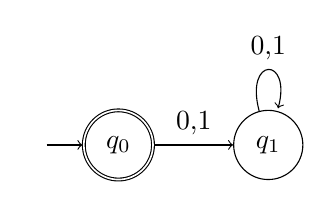
\begin{tikzpicture}
                   \node[state,initial,accepting] (q_0)   {$q_0$};
                   \node[state] (q_1) [right=of q_0] {$q_1$};
                    \path[->]
                    (q_0) edge [above] node {0,1} (q_1)
                    (q_1) edge [loop above] node {0,1} (q_1);
                \end{tikzpicture}
                \\
            \item
                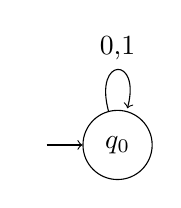
\begin{tikzpicture}
                   \node[state,initial] (q_0)   {$q_0$};
                    \path[->]
                    (q_0) edge [loop above] node {0,1} (q_0);
                \end{tikzpicture}
                \\
            \item
                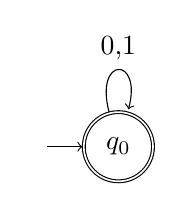
\begin{tikzpicture}
                   \node[state,initial,accepting] (q_0)   {$q_0$};
                    \path[->]
                    (q_0) edge [loop above] node {0,1} (q_0);
                \end{tikzpicture}
        \end{enumerate}
    \item % 2
        \begin{enumerate}
            \item
                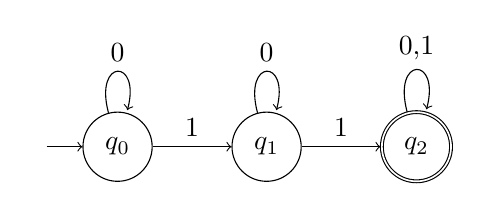
\begin{tikzpicture}
                   \node[state,initial] (q_0)   {$q_0$};
                   \node[state] (q_1) [right=of q_0] {$q_1$};
                   \node[state,accepting] (q_2) [right=of q_1] {$q_2$};
                    \path[->]
                    (q_0) edge [loop above] node {0} (q_0)
                          edge [above] node {1} (q_1)
                    (q_1) edge [loop above] node {0} (q_1)
                          edge [above] node {1} (q_2)
                    (q_2) edge [loop above] node {0,1} (q_2);
                \end{tikzpicture}
                \\
            \item
                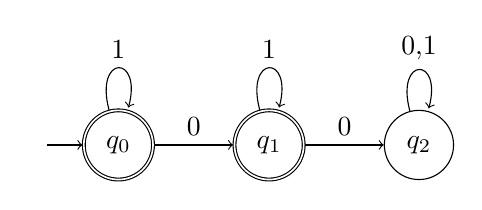
\begin{tikzpicture}
                   \node[state,initial,accepting] (q_0)   {$q_0$};
                   \node[state,accepting] (q_1) [right=of q_0] {$q_1$};
                   \node[state] (q_2) [right=of q_1] {$q_2$};
                    \path[->]
                    (q_0) edge [above] node {0} (q_1)
                          edge [loop above] node {1} (q_0)
                    (q_1) edge [above] node {0} (q_2)
                          edge [loop above] node {1} (q_1)
                    (q_2) edge [loop above] node {0,1} (q_2);
                \end{tikzpicture}
                \\
            \item
                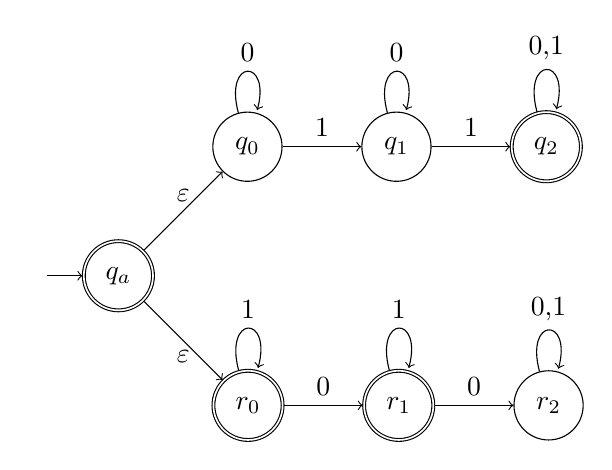
\begin{tikzpicture}
                   \node[state,initial,accepting] (q_a)   {$q_a$};
                   \node[state] (q_0) [above right=of q_a] {$q_0$};
                   \node[state] (q_1) [right=of q_0] {$q_1$};
                   \node[state,accepting] (q_2) [right=of q_1] {$q_2$};
                   \node[state,accepting] (r_0) [below right=of q_a]  {$r_0$};
                   \node[state,accepting] (r_1) [right=of r_0] {$r_1$};
                   \node[state] (r_2) [right=of r_1] {$r_2$};
                    \path[->]
                    (q_a) edge [above] node {$\varepsilon$} (q_0)
                          edge [below] node {$\varepsilon$} (r_0)
                    (q_0) edge [loop above] node {0} (q_0)
                          edge [above] node {1} (q_1)
                    (q_1) edge [loop above] node {0} (q_1)
                          edge [above] node {1} (q_2)
                    (q_2) edge [loop above] node {0,1} (r_2)
                    (r_0) edge [above] node {0} (r_1)
                          edge [loop above] node {1} (r_0)
                    (r_1) edge [above] node {0} (r_2)
                          edge [loop above] node {1} (q_1)
                    (r_2) edge [loop above] node {0,1} (r_2);
                \end{tikzpicture}
        \end{enumerate}
    \item % 3

    \item % 4
    \item % 5
    \item % 6
\end{enumerate}

\end{document}
